\chapter{无穷级数}
无穷级数是高等数学的一个重要组成部分;
它是表示函数,研究函数性质,以及进行数值计算的一种工具.
本章先讨论常数项级数,介绍无穷级数的一些基本内容,然后讨论函数项级数,
着重讨论如何将函数展开成幂级数和三角级数的问题.

\section{常数项级数的概念和性质}
人们认识事物在数量方面的特性,往往有一个由近似到精确的过程.
在这种认识过程中,会遇到由有限个数量相加到无穷多个数量相加的问题.

例如计算半径为\(R\)的圆面积\(A\),具体做法如下:
如\cref{figure:无穷级数.用内接正多边形覆盖圆},
作圆的内接正六边形,算出这六边形的面积\(a_1\),它是圆面积\(A\)的一个粗糙的近似值.
为了比较准确地计算出\(A\)的值,
我们以这个正六边形的每一边为底分别作一个顶点在圆周上的等腰三角形,
算出这六个等腰三角形的面积之和\(a_2\).
那么\(a_1+a_2\)(即内接正十二边形的面积)就是\(A\)的一个较好的近似值.
同样地,在这正十二边形的每一边上分别作一个顶点在圆周上的等腰三角形,
算出这十二个等腰三角形的面积之和\(a_3\).
那么\(a_1+a_2+a_3\)(即内接正二十四边形的面积)是\(A\)的一个更好的近似值.
如此继续下去,内接\(3\cdot2^n\)边形的面积就逐步逼近圆面积:\[
	A \approx a_1 + a_2 + \dotsb + a_n.
\]

\begin{figure}[h]
	\centering
	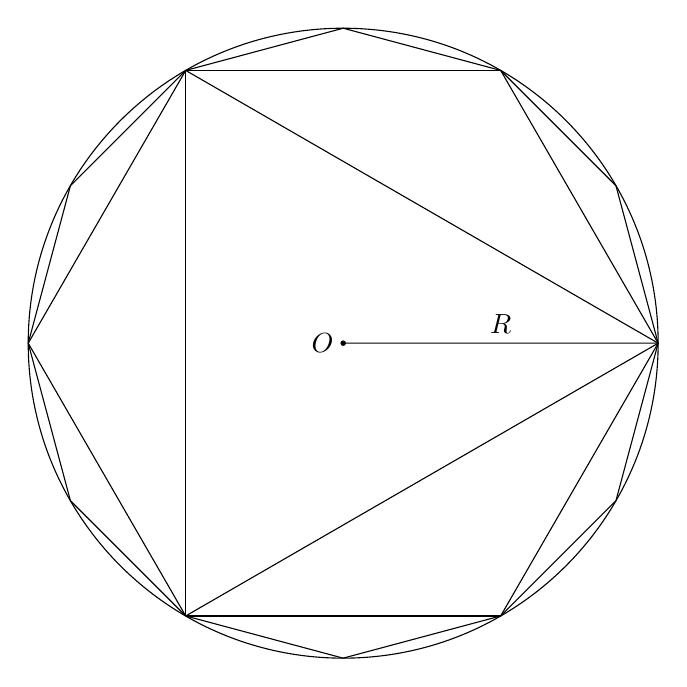
\begin{tikzpicture}
		\pgfmathsetmacro{\radius}{4}
		\def\PlotPolygon#1{
			\foreach \i in {1,...,#1}{
				\draw({\radius*cos(\i*360/#1)},{\radius*sin(\i*360/#1)})
				--({\radius*cos((\i-1)*360/#1)},{\radius*sin((\i-1)*360/#1)});
			}
		}
		\begin{scope}
			\PlotPolygon{3}
			\PlotPolygon{6}
			\PlotPolygon{12}
		\end{scope}
		\draw(0,0)circle(\radius)node[left]{\(O\)}
			--(\radius,0)node[midway,above]{\(R\)};
		\fill(0,0)circle(1pt);

	\end{tikzpicture}
	\caption{用内接正多边形覆盖圆}
	\label{figure:无穷级数.用内接正多边形覆盖圆}
\end{figure}

如果内接正多边形的边数无限增多,即\(n\)无限增大,
则和\(a_1+a_2+\dotsb+a_n\)的极限就是所要求的圆面积\(A\).
这时和式中的项数无限增多,于是出现了无穷多个数量依次相加的数学式子.

\subsection{常数项级数的概念}
\begin{definition}\label{definition:无穷级数.常数项级数的定义}
一般地,给定一个有无穷多项的数列\[
	u_1,u_2,\dotsc,u_n,\dotsc,
\]
则由该数列构成的表达式\[
	u_1+u_2+\dotsb+u_n+\dotsb
\]
叫做\DefineConcept{常数项无穷级数}(infinite series with constant terms),
简称\DefineConcept{常数项级数},
记作\(\sum\limits_{n=1}^\infty u_n\),
即\[
	\sum\limits_{n=1}^\infty u_n
	\defeq
	u_1+u_2+\dotsb+u_n+\dotsb,
\]
其中第\(n\)项\(u_n\)叫做级数的\DefineConcept{一般项}.

作常数项级数的前\(n\)项的和\[
	s_n = u_1+u_2+\dotsb+u_n = \sum\limits_{i=1}^n{u_i}.
\]
我们把\(s_n\)称为级数\(\sum\limits_{n=1}^\infty u_n\)的\DefineConcept{部分和}(partial sum).

如果级数\(\sum\limits_{n=1}^\infty u_n\)的部分和数列\(\{s_n\}\)有极限\(s\),即\[
	\lim\limits_{n\to\infty} s_n = s,
\]
则称“无穷级数\(\sum\limits_{n=1}^\infty u_n\) \DefineConcept{收敛}(converge)”,
这时极限\(s\)叫做这级数的\DefineConcept{和}(sum),并写成\[
	s = u_1+u_2+\dotsb+u_n+\dotsb;
\]
反之,如果\(\{s_n\}\)没有极限,
则称“无穷级数\(\sum\limits_{n=1}^\infty u_n\) \DefineConcept{发散}(diverge)”.

显然,当级数收敛时,其部分和\(s_n\)是级数的和\(s\)的近似值,它们之间的差值\[
	r_n = s - s_n = u_{n+1}+u_{n+2}+\dotsb
\]
叫做“级数\(\sum\limits_{n=1}^\infty u_n\)的\DefineConcept{余项}”.
称这个余项的绝对值\(\abs{r_n}\)为%
“用近似值\(s_n\)代替和\(s\)所产生的\DefineConcept{误差}”.
\end{definition}
从上述定义可知,级数与数列极限有着紧密的联系.给定级数\(\sum\limits_{n=1}^\infty u_n\),
就有部分和数列\(\{s_n = \sum\limits_{i=1}^n u_n\}\);
反之,给定数列\(\{s_n\}\),就有以\(\{s_n\}\)为部分和数列的级数\[
	s_1 + (s_2-s_1) + \dotsb + (s_n-s_{n-1}) + \dotsb
	= s_1 + \sum\limits_{i=2}^\infty (s_i-s_{i-1})
	= \sum\limits_{n=1}^\infty u_n,
\]
其中\(u_1=s_1\),\(u_n=s_n-s_{n-1}\ (n \geq 2)\).
按定义,级数\(\sum\limits_{n=1}^\infty u_n\)与数列\(\{s_n\}\)同时收敛或同时发散,
且在收敛时,有\[
	\sum\limits_{n=1}^\infty u_n = \lim\limits_{n\to\infty} s_n,
\]
即\(\sum\limits_{n=1}^\infty u_n = \lim\limits_{n\to\infty} \sum\limits_{i=1}^n u_n\).

\begin{example}\label{example:无穷级数.等比级数的收敛性}
无穷级数\[
	\sum\limits{n=1} a q^n
	= a+aq+aq^2+\dotsb+aq^n+\dotsb
\]
叫做\DefineConcept{等比级数}或\DefineConcept{几何级数},
其中\(a \neq 0\),\(q\)叫做\DefineConcept{级数的公比}.
试讨论上述等比级数的收敛性.
\begin{solution}
当\(q = 1\)时,则部分和\(s_n=na\),那么\(\lim\limits_{n\to\infty} s_n = \lim\limits_{n\to\infty} na = \infty\),即级数发散.

当\(q \neq 1\),则\[
s_n = \frac{a(1-q^n)}{1-q} = \frac{a}{1-q} - \frac{aq^n}{1-q}.
\]
当\(\abs{q} < 1\)时由于\(\lim\limits_{n\to\infty} q^n=0\),从而\(\lim\limits_{n\to\infty} s_n=\frac{a}{1-q}\),
因此级数收敛,其和为\(\frac{a}{1-q}\).
当\(\abs{q} > 1\)时由于\(\lim\limits_{n\to\infty} q^n=\infty\),从而\(\lim\limits_{n\to\infty} s_n=\infty\),即级数发散.
当\(q = -1\)时,级数变为\(a-a+a-a+\dotsb\),
显然\(s_n\)随着\(n\)为奇数或为偶数而等于\(a\)或等于零,从而\(s_n\)的极限不存在,这是级数也发散.

综上所述,{\color{red}当\(\abs{q} < 1\)时,几何级数收敛;当\(\abs{q} \geq 1\)时,几何级数发散.}
\end{solution}
\end{example}

\begin{example}\label{example:无穷级数.等差级数的收敛性}
试证级数\[
1+2+3+\dotsb+n+\dotsb
\]是发散的.
\begin{proof}
级数的部分和为\[
s_n = 1+2+3+\dotsb+n = \frac{n(n+1)}{2}.
\]显然,\(\lim\limits_{n\to\infty} s_n=\infty\),级数是发散的.
\end{proof}
\end{example}
从上例也可看出:
\begin{proposition}
除非初项\(a_0\)与公差\(d\)都等于\(0\),
否则等差级数\(\sum\limits_{n=0}^\infty(a_0+nd)\)总是发散的.
\end{proposition}

\begin{example}
判定无穷级数\[
\frac{1}{1\cdot2}+\frac{1}{2\cdot3}+\dotsb+\frac{1}{n(n+1)}+\dotsb
\]的收敛性.
\begin{solution}
记\[
	u_n = \frac{1}{n(n+1)} = \frac{1}{n}-\frac{1}{n+1},
\]
因此\begin{align*}
	s_n &= \frac{1}{1\cdot2}+\frac{1}{2\cdot3}+\dotsb+\frac{1}{n(n+1)} \\
	&= \left(1-\frac{1}{2}\right)+\left(\frac{1}{2}-\frac{1}{3}\right)
	+\dotsb+\left(\frac{1}{n}-\frac{1}{n+1}\right) \\
	&= 1-\frac{1}{n+1}.
\end{align*}
从而\[
	\lim\limits_{n\to\infty} s_n = \lim\limits_{n\to\infty} \left(1-\frac{1}{n+1}\right) = 1,
\]
即该级数收敛,它的和为\(1\).
\end{solution}
\end{example}

\subsection{收敛级数的基本性质}
\begin{property}\label{theorem:无穷级数.收敛级数性质1}
如果级数\(\sum\limits_{n=1}^\infty u_n\)收敛于和\(s\),
则级数\(\sum\limits_{n=1}^\infty k u_n\)收敛于和\(ks\).
\begin{proof}
设级数\(\sum\limits_{n=1}^\infty u_n\)
与级数\(\sum\limits_{n=1}^\infty k u_n\)的
部分和分别为\(s_n\)与\(\sigma_n\),
则\[
	\sigma_n
	= k u_1 + k u_2 + \dotsb + k u_n
	= k(u_1 + u_2 + \dotsb + u_n) = k s_n,
\]\[
	\lim\limits_{n\to\infty} \sigma_n
	= \lim\limits_{n\to\infty} k s_n
	= k \lim\limits_{n\to\infty} s_n = ks,
\]
也就是说,级数\(\sum\limits_{n=1}^\infty k u_n\)收敛于\(ks\).

特别地,对于任意发散级数\(\sum\limits_{n=1}^\infty u_n\),
级数\(\sum\limits_{n=1}^\infty 0 \cdot u_n\)的每一项都是零,
故级数\(\sum\limits_{n=1}^\infty 0 \cdot u_n\)收敛于\(0\).
\end{proof}
\end{property}

由关系式\(\sigma_n = k s_n\)知道,
如果\(\{s_n\}\)没有极限且\(k\neq0\),
那么\(\{\sigma_n\}\)也不可能有极限.
因此我们得到如下结论:
{\color{red}级数的每一项同乘一个非零常数后,它的敛散性不会改变.}

\begin{example}
判断\[
\sin\frac{\pi}{6}+\sin\frac{2\pi}{6}+\dotsb+\sin\frac{n\pi}{6}+\dotsb
\]的收敛性.
\begin{solution}
记\(u_n = \sin\frac{n\pi}{6},
v_n = 2\sin\frac{\pi}{12} \cdot u_n\).
因为\[
	v_n = \cos\frac{\pi-2n\pi}{12} - \cos\frac{\pi+2n\pi}{12},
\]\[
	\sigma_n
	= v_1 + v_2 + \dotsb + v_n
	= \cos\frac{\pi}{12} - \cos\frac{(2n+1)\pi}{12},
\]
所以\[
	s_n
	= \left(2\sin\frac{\pi}{12}\right)^{-1} \cdot \sigma_n
	= 1+\frac{\sqrt{3}}{2} - \frac{\sqrt{2}}{\sqrt{3}-1} \cos\frac{(2n+1)\pi}{12}.
\]
可见\(\lim\limits_{n\to\infty} s_n\)不存在,级数发散.
\end{solution}
\end{example}

\begin{property}\label{theorem:无穷级数.收敛级数性质2}
如果级数\(\sum\limits_{n=1}^\infty u_n\)、\(\sum\limits_{n=1}^\infty v_n\)分别收敛于\(s\)、\(\sigma\),
则级数\(\sum\limits_{n=1}^\infty(u_n \pm v_n)\)收敛于\(s \pm \sigma\).
\begin{proof}
设级数\(\sum\limits_{n=1}^\infty u_n\)与级数\(\sum\limits_{n=1}^\infty v_n\)的部分和分别为\(s_n\)与\(\sigma_n\),
则级数\(\sum\limits_{n=1}^\infty(u_n \pm v_n)\)的部分和\begin{align*}
	\tau_n &= (u_1 \pm v_1) + (u_2 \pm v_2) + \dotsb + (u_n + v_n) \\
	&= (u_1 + u_2 + \dotsb + u_n) \pm (v_1 + v_2 + \dotsb + v_n) \\
	&= s_n \pm \sigma_n,
\end{align*}
于是\[
	\lim\limits_{n\to\infty} \tau_n
	= \lim\limits_{n\to\infty} (s_n \pm \sigma_n)
	= s + \sigma.
\]

这就表明级数\(\sum\limits_{n=1}^\infty(u_n \pm v_n)\)收敛于\(s \pm \sigma\).
\end{proof}
\end{property}
\cref{theorem:无穷级数.收敛级数性质2} 也可以说成:
{\color{red}两个收敛级数可以逐项相加、逐项相减.}

\begin{example}
设级数\(\sum\limits_{n=1}^\infty u_n\)收敛,\(\sum\limits_{n=1}^\infty v_n\)发散.
试证:级数\(\sum\limits_{n=1}^\infty (u_n \pm v_n)\)发散.
\begin{proof}
设级数\(\sum\limits_{n=1}^\infty u_n\)与\(\sum\limits_{n=1}^\infty v_n\)的部分和分别为\(s_n\)和\(\sigma_n\),又设\[
\lim\limits_{n\to\infty} s_n = s.
\]
假设级数\(\sum\limits_{n=1}^\infty (u_n \pm v_n)\)收敛,且\[
\lim\limits_{n\to\infty} (s_n \pm \sigma_n) = s+\sigma,
\]那么根据\hyperref[theorem:极限.极限的四则运算法则]{极限的四则运算法则}\[
\lim\limits_{n\to\infty} \pm\sigma_n
= \lim\limits_{n\to\infty} [(s_n \pm \sigma_n) - s_n]
= \lim\limits_{n\to\infty} (s_n \pm \sigma_n) - \lim\limits_{n\to\infty} s_n
= (s + \sigma) - s
= \sigma,
\]也就是说\(\{\pm\sigma_n\}\)(即\(\pm\sum\limits_{n=1}^\infty v_n\))收敛,矛盾!
\end{proof}
\end{example}
从上例我们可以看出:
{\color{red}一个收敛级数与一个发散级数相加(或相减)所得级数必定发散.}

另一方面,任给一个发散级数\(\sum\limits_{n=1}^\infty u_n\),
级数\(\sum\limits_{n=1}^\infty u_n + \sum\limits_{n=1}^\infty u_n
= \sum\limits_{n=1}^\infty 2 u_n\)也是发散的,
而级数\(\sum\limits_{n=1}^\infty u_n - \sum\limits_{n=1}^\infty u_n
= 0\)却是收敛的,
于是我们还可以看出:
{\color{red}两个发散级数相加(或相减)所得级数可能收敛也可能发散.}

\begin{example}
已知级数\(\sum\limits_{n=1}^\infty (-1)^{n-1} a_n = 2,
\sum\limits_{n=1}^\infty a_{2n-1} = 5\),
求\(\sum\limits_{n=1}^\infty a_n\).
\begin{solution}
由于\(\sum\limits_{n=1}^\infty [a_n + (-1)^{n-1} a_n]
= 2 \sum\limits_{n=1}^\infty a_{2n-1}\)收敛,
所以\(\sum\limits_{n=1}^\infty a_n\)收敛,且有
\[
\sum\limits_{n=1}^\infty a_n
= 2 \sum\limits_{n=1}^\infty a_{2n-1}
- \sum\limits_{n=1}^\infty (-1)^{n-1} a_n
= 10 - 2 = 8.
\]
\end{solution}
\end{example}

\begin{property}\label{theorem:无穷级数.收敛级数性质3}
在级数中去掉、加上或改变有限项,不会改变级数的收敛性.
\begin{proof}
我们只需证明“在级数的前面部分去掉或加上有限项,不会改变级数的收敛性”,
因为其他情形(即在级数中任意去掉、加上或改变有限项的情形)都可以看成在级数的前面部分先去掉有限项,
然后再加上有限项的结果.

将级数\[
u_1+u_2+\dotsb+u_k+u_{k+1}+\dotsb+u_{k+n}+\dotsb
\]的前\(k\)项去掉,则得级数\[
u_{k+1}+u_{k+2}+\dotsb+u_{k+n}+\dotsb.
\]于是新得到的级数的部分和为\[
\sigma_n = u_{k+1}+u_{k+2}+\dotsb+u_{k+n} = s_{k+n} - s_k,
\]其中\(s_{k+n}\)是原级数的前\(k+n\)项的和.
因为\(s_k\)是常数,所以当\(n\to\infty\)时,
\(\sigma_n\)与\(s_{k+n}\)这两个量,要么同时具有极限,要么同时没有极限.

同理可证在级数的前面加上有限项,不会改变级数的收敛性.
由此可见,在级数中去掉、加上或改变有限项,不会改变级数的收敛性.

另外,我们可以观察到,在收敛级数中去掉、加上或改变有限项,
虽不会改变级数的收敛性,但可能会改变收敛级数的和.
\end{proof}
\end{property}

\begin{property}\label{theorem:无穷级数.收敛级数性质4}
如果级数\(\sum\limits_{n=1}^\infty u_n\)收敛,则对这级数的项任意加括号后所成的级数\[
(u_1+\dotsb+u_{n_1}) + (u_{n_1+1}+\dotsb+u_{n_2}) + \dotsb + (u_{n_{k-1}+1}+\dotsb+u_{n_k}) + \dotsb
\]仍收敛,且其和不变.
\end{property}

应该注意到:
如果加括号后所成的级数收敛,则不能断定去括号后原来的级数也收敛.
例如,级数\[
(1-1)+(1-1)+\dotsb
\]收敛于零,但级数\[
1-1+1-1+\dotsb
\]却是发散的.

根据\cref{theorem:无穷级数.收敛级数性质4} 可得如下推论:{\color{red}如果加括号后所成的级数发散,则原来的级数也发散.}
事实上,倘若原级数收敛,则根据\cref{theorem:无穷级数.收敛级数性质4} 知道,加括号后的级数就应该收敛了.

\begin{property}[级数收敛的必要条件]\label{theorem:无穷级数.收敛级数性质5}
如果级数\(\sum\limits_{n=1}^\infty u_n\)收敛,则它的一般项\(u_n\)满足\[
\lim\limits_{n\to\infty} u_n = 0.
\]
\begin{proof}
设级数\(\sum\limits_{n=1}^\infty u_n\)的部分和为\(s_n\),且\(\lim\limits_{n\to\infty} s_n = s\),则\[
\lim\limits_{n\to\infty} u_n = \lim\limits_{n\to\infty}(s_n - s_{n-1}) = \lim\limits_{n\to\infty} s_n - \lim\limits_{n\to\infty} s_{n-1} = s - s = 0.
\qedhere
\]
\end{proof}
\end{property}

根据\cref{theorem:无穷级数.收敛级数性质5} 可知,如果\(\lim\limits_{n\to\infty} u_n \neq 0\),那么\(\sum\limits_{n=1}^\infty u_n\)一定发散.
例如,级数\[
\frac{1}{2}-\frac{2}{3}+\frac{3}{4}-\dotsb+(-1)^{n-1}\frac{n}{n+1}+\dotsb,
\]它的一般项\(u_n = (-1)^{n-1} \frac{n}{n+1}\)当\(n\to\infty\)时不趋于零,因此该级数是发散的.

值得注意的是,级数的一般项趋于零并不是级数收敛的充分条件.
有些级数虽然一般项趋于零,但仍然是发散的.
\begin{example}\label{example:无穷级数.调和级数的收敛性}
试证:调和级数\[
\sum\limits_{n=1}^\infty u_n = 1+\frac{1}{2}+\frac{1}{3}+\dotsb+\frac{1}{n}+\dotsb
\]是发散的.
\begin{proof}
虽然调和级数的一般项\(\lim\limits_{n\to\infty} u_n = \lim\limits_{n\to\infty} 1/n = 0\),但是它是发散的.
现在我们用反证法证明.

假设级数\(\sum\limits_{n=1}^\infty u_n\)收敛.设级数的部分和为\(s_n\),且\(\lim\limits_{n\to\infty} s_n = s\).
显然,对级数\(\sum\limits_{n=1}^\infty u_n\)的部分和\(s_{2n}\)也有\(\lim\limits_{n\to\infty} s_{2n} = s\).
于是\[
\lim\limits_{n\to\infty} {s_{2n}-s_n} = \lim\limits_{n\to\infty} s_{2n} - \lim\limits_{n\to\infty} s_n = s - s = 0.
\]但另一方面\[
s_{2n} - s_n = \frac{1}{n+1}+\frac{1}{n+2}+\dotsb+\frac{1}{2n}
> \underbrace{\frac{1}{2n}+\frac{1}{2n}+\dotsb+\frac{1}{2n}}_{n\text{项}}
= \frac{1}{2},
\]\[
\lim\limits_{n\to\infty} {s_{2n}-s_n} \neq 0,
\]与假设矛盾,说明级数\(\sum\limits_{n=1}^\infty u_n\)必定发散.
\end{proof}
\end{example}

\subsection{柯西审敛原理}
\begin{theorem}[柯西审敛原理]\label{theorem:无穷级数.级数的柯西审敛原理}
级数\(\sum\limits_{n=1}^\infty u_n\)收敛的充要条件为:
对于任意给定的正数\(\epsilon\),总存在正整数\(N\),
使得当\(n>N\)时,对于任意的正整数\(p\),都有\[
\abs{ \sum\limits_{i=1}^p u_{n+i} }
= \abs{u_{n+1}+u_{n+2}+\dotsb+u_{n+p}}
< \epsilon
\]成立.
\begin{proof}
设级数\(\sum\limits_{n=1}^\infty u_n\)的部分和为\(s_n\),因为\[
\abs{u_{n+1}+u_{n+2}+\dotsb+u_{n+p}} = \abs{s_{n+p}-s_n},
\]所以由\hyperref[theorem:极限.数列的柯西极限存在准则]{柯西极限存在准则}可得本定理结论.
\end{proof}
\end{theorem}

\begin{example}
试求级数\(\sum\limits_{n=1}^\infty \frac{1}{n^2}\)的收敛性.
\begin{solution}
因为对任意正整数\(p\),\begin{align*}
&\abs{u_{n+1}+u_{n+2}+\dotsb+u_{n+p}} \\
&=\frac{1}{(n+1)^2}+\frac{1}{(n+2)^2}+\dotsb+\frac{1}{(n+p)^2} \\
&<\frac{1}{n(n+1)}+\frac{1}{(n+1)(n+2)}+\dotsb+\frac{1}{(n+p-1)(n+p)} \\
&=\left(\frac{1}{n}-\frac{1}{n+1}\right)+\left(\frac{1}{n+1}-\frac{1}{n+2}\right)+\dotsb+\left(\frac{1}{n+p-1}-\frac{1}{n+p}\right) \\
&=\frac{1}{n}-\frac{1}{n+p} < \frac{1}{n},
\end{align*}
所以对于\(\forall \epsilon > 0\),取正整数\(N \geq \frac{1}{\epsilon}\),则当\(n > N\)时,对任何正整数\(p\),都有\[
\abs{u_{n+1}+u_{n+2}+\dotsb+u_{n+p}}
< \frac{1}{n}
< \frac{1}{N}
\leq \epsilon
\]成立.
按柯西审敛原理,级数\(\sum\limits_{n=1}^\infty \frac{1}{n^2}\)收敛.
\end{solution}
\end{example}

\section{常数项级数的审敛法}
\subsection{正项级数及其审敛法}
\subsubsection{正项级数的概念及其收敛条件}
一般的常数项级数,它的各项可以是正数、负数或零.
现在我们先讨论各项都是正数或零的级数,这种级数称为\DefineConcept{正项级数}.
这种级数特别重要,以后将看到许多级数的收敛性问题可归结为正项级数的收敛性问题.

\begin{theorem}\label{theorem:无穷级数.正项级数收敛的充要条件}
%@see: 《高等数学(第六版 下册)》 P256. 定理1
%@see: 《数学分析教程 (第三版 下册)》 P163. 定理14.2.1
正项级数\(\sum\limits_{n=1}^\infty u_n\)收敛的充要条件是:
它的部分和数列\(\{s_n\}\)有界.
\begin{proof}
显然,数列\(\{s_n\}\)是一个单调增加数列.
如果数列\(\{s_n\}\)有界,
那么根据\hyperref[theorem:极限.数列的单调有界定理]{单调有界定理},
数列\(\{s_n\}\)收敛,
也就是说,级数\(\sum\limits_{n=1}^\infty u_n\)收敛.

反之,如果正项级数\(\sum\limits_{n=1}^\infty u_n\)收敛于和\(s\),
即\(\lim\limits_{n\to\infty} s_n = s\),
根据\hyperref[theorem:极限.收敛数列的有界性]{收敛数列的有界性}可知,
数列\(\{s_n\}\)有界.
\end{proof}
\end{theorem}

我们可以写出\cref{theorem:无穷级数.正项级数收敛的充要条件} 的逆否命题.
\begin{proposition}
正项级数\(\sum\limits_{n=1}^\infty u_n\)发散的充要条件是它的部分和数列无界.
\end{proposition}

\begin{example}
%@see: 《数学分析教程 (第三版 下册)》 P163. 例1
设正项级数\(\sum\limits_{n=1}^\infty a_n\)的部分和是\(s_n\),证明:\[
	\sum\limits_{n=1}^\infty \frac{a_n}{s_n^2} < +\infty.
\]
\begin{proof}
显然\(\sum\limits_{n=1}^\infty \frac{a_n}{s_n^2}\)是正项级数.
由于对于任意正整数\(N\),有\begin{align*}
	\sum_{n=2}^N \frac{a_n}{s_n^2}
	&= \sum_{n=2}^N \frac{s_n-s_{n-1}}{s_n^2}
	\leq \sum_{n=2}^N \frac{s_n-s_{n-1}}{s_{n-1} s_n} \\
	&= \sum_{n=2}^N \left(
			\frac{1}{s_{n-1}} - \frac{1}{s_n}
		\right)
	= \frac{1}{s_1} - \frac{1}{s_N}
	< \frac{1}{a_1},
\end{align*}
也就是说\(\sum\limits_{n=1}^\infty \frac{a_n}{s_n^2}\)的部分和有界,
所以根据\cref{theorem:无穷级数.正项级数收敛的充要条件},该级数收敛.
\end{proof}
\end{example}

\begin{example}
设正项级数\(\sum\limits_{n=1}^\infty a_n\)的部分和是\(s_n\),
证明:对于任意\(k>1\),有\[
	\sum_{n=1}^\infty \frac{a_n}{s_n^k} < +\infty.
\]
%TODO
\end{example}

\subsubsection{比较审敛法}
利用\cref{theorem:无穷级数.正项级数收敛的充要条件} 直接证明某些级数的部分和有界不太容易,
因此我们需要一个判别级数敛散性的更简单的方法.

\begin{theorem}[比较审敛法]\label{theorem:无穷级数.正项级数的比较审敛法}
%@see: 《高等数学(第六版 下册)》 P256. 定理2
%@see: 《数学分析教程 (第三版 下册)》 P164. 定理14.2.2
设\(\sum\limits_{n=1}^\infty u_n\)
和\(\sum\limits_{n=1}^\infty v_n\)都是正项级数,且\[
	u_n \leq v_n
	\quad(n=1,2,\dotsc).
\]
若级数\(\sum\limits_{n=1}^\infty v_n\)收敛,
则级数\(\sum\limits_{n=1}^\infty u_n\)收敛;
反之,若级数\(\sum\limits_{n=1}^\infty u_n\)发散,
则级数\(\sum\limits_{n=1}^\infty v_n\)发散.
\begin{proof}
设级数\(\sum\limits_{n=1}^\infty v_n\)收敛于和\(\sigma\),
则级数\(\sum\limits_{n=1}^\infty u_n\)的部分和\[
	s_n = u_1 + u_2 + \dotsb u_n
	\leq
	v_1 + v_2 + \dotsb + v_n \leq \sigma
	\quad(n=1,2,\dotsc),
\]
即部分和数列\(\{s_n\}\)有界,
由\cref{theorem:无穷级数.正项级数收敛的充要条件} 知级数\(\sum\limits_{n=1}^\infty u_n\)收敛.
\end{proof}
\end{theorem}

\begin{example}
判断级数\(\sum\limits_{n=1}^\infty \frac{1}{1+a^n}\ (a>0)\)的收敛性.
\begin{solution}
显然有\[
	\frac{1}{1+a^n} < \frac{1}{a^n}.
\]
根据比较审敛法,如果级数\(\sum\limits_{n=1}^\infty \frac{1}{a^n}\)收敛,
那么级数\(\sum\limits_{n=1}^\infty \frac{1}{1+a^n}\)收敛;
而等比级数\(\sum\limits_{n=1}^\infty \frac{1}{a^n}\)
当且仅当其公比\(\abs{\frac{1}{a}} < 1\),即\(a > 1\)时收敛;
故当\(a > 1\)时,级数\(\sum\limits_{n=1}^\infty \frac{1}{1+a^n}\)收敛.

当\(0 < a \leq 1\)时,\(0 < a^n \leq 1\),\(1 < 1 + a^n \leq 2\),\[
	\frac{1}{1+a^n} \geq \frac{1}{2},
\]
而等差级数\(\sum\limits_{n=1}^\infty \frac{1}{2}\)发散,
故级数\(\sum\limits_{n=1}^\infty \frac{1}{1+a^n}\)发散.
\end{solution}
\end{example}

注意到级数的每一项同乘不为零的常数\(k\)
以及去掉级数前面部分的有限项不会影响级数的收敛性,
我们可得如下推论:
\begin{corollary}\label{theorem:无穷级数.正项级数的比较审敛法的推论}
设\(\sum\limits_{n=1}^\infty u_n\)和\(\sum\limits_{n=1}^\infty v_n\)都是正项级数.
如果级数\(\sum\limits_{n=1}^\infty v_n\)收敛,且存在正整数\(N\),
使当\(n \geq N\)时有\(u_n \leq k v_n\ (k > 0)\)成立,
则级数\(\sum\limits_{n=1}^\infty u_n\)收敛;
如果级数\(\sum\limits_{n=1}^\infty v_n\)发散,且存在正整数\(N\),
使当\(n \geq N\)时有\(u_n \geq k v_n\ (k > 0)\)成立,
则级数\(\sum\limits_{n=1}^\infty u_n\)发散.
\end{corollary}

\begin{example}
试证:级数\(\sum\limits_{n=1}^\infty \frac{1}{\sqrt{n(n+1)}}\)是发散的.
\begin{proof}
因为\(n(n+1) < (n+1)^2\),所以\(\frac{1}{\sqrt{n(n+1)}} > \frac{1}{n+1}\),而级数\(\sum\limits_{n=1}^\infty \frac{1}{n+1}\)是发散的,根据比较审敛法可知级数\(\sum\limits_{n=1}^\infty \frac{1}{\sqrt{n(n+1)}}\)是发散的.
\end{proof}
\end{example}

\subsubsection{p级数}
\begin{example}\label{example:无穷级数.p级数的收敛性}
讨论p级数\[
1+\frac{1}{2^p}+\frac{1}{3^p}+\dotsb+\frac{1}{n^p}+\dotsb
\]的收敛性,其中常数\(p>0\).
\begin{solution}
当\(p \leq 1\)时,p级数各项均不小于调和级数对应项,即\(\frac{1}{n^p} \geq \frac{1}{n}\),但调和级数发散,故根据\cref{theorem:无穷级数.正项级数的比较审敛法} 可知,当\(p \leq 1\)时p级数发散.

当\(p > 1\)时,因为\(k-1 \leq x \leq k \implies \frac{1}{k} \leq \frac{1}{x} \implies \frac{1}{k^p} \leq \frac{1}{x^p}\),所以\[
\frac{1}{k^p}
= \int_{k-1}^k \frac{1}{k^p} \dd{x}
\leq \int_{k-1}^k \frac{1}{x^p} \dd{x}
\quad(k=2,3,\dotsc),
\]
从而级数的部分和
\begin{align*}
s_n &= 1 + \sum\limits_{k=2}^n{\frac{1}{k^p}}
\leq 1 + \sum\limits_{k=2}^n{ \int_{k-1}^k{\frac{1}{x^p}\dd{x}} }
= 1 + \int_1^n{\frac{1}{x^p}\dd{x}} \\
&= 1 + \frac{1}{p-1}\left(1-\frac{1}{n^{p-1}}\right)
< 1 + \frac{1}{p-1}
\quad(n=2,3,\dotsc),
\end{align*}
这表明数列\(\{s_n\}\)有界,因此p级数收敛.

综上所述,{\color{red} p级数\(\sum\limits_{n=1}^\infty \frac{1}{n^p}\)当\(p > 1\)时收敛,当\(p \leq 1\)时发散.}
\end{solution}
\end{example}
可以发现,p级数与\hyperref[example:定积分.p积分]{p积分}具有高度相似性.

\begin{example}
设正项级数\(\sum\limits_{n=1}^\infty a_n\)发散,证明:级数\(\sum\limits_{n=1}^\infty \frac{a_n}{n^3+a_n^2}\)收敛.
\begin{proof}
由基本不等式 \labelcref{theorem:不等式.基本不等式1} 可知
\(n^3+a_n^2\geq2\sqrt{n^3 a_n^2}=2n^{3/2}a_n\),
那么\(\frac{a_n}{n^3+a_n^2}\leq\frac{a_n}{2n^{3/2}a_n}=\frac{1}{2n^{3/2}}\).
由\cref{example:无穷级数.p级数的收敛性}
我们知道\(p=\frac{3}{2}>1\)时,p级数收敛;
那么根据\hyperref[theorem:无穷级数.正项级数的比较审敛法]{比较审敛法}可知
级数\(\sum\limits_{n=1}^\infty \frac{a_n}{n^3+a_n^2}\)收敛.
\end{proof}
\end{example}

\subsubsection{比较审敛法的极限形式}
\begin{theorem}[比较审敛法的极限形式]\label{theorem:无穷级数.正项级数的比较审敛法的极限形式}
设\(\sum\limits_{n=1}^\infty u_n\)和\(\sum\limits_{n=1}^\infty v_n\)都是正项级数,记\[
l = \lim\limits_{n\to\infty} \frac{u_n}{v_n}.
\]\begin{enumerate}
\item 如果\(l\in[0,+\infty)\),且级数\(\sum\limits_{n=1}^\infty v_n\)收敛,则级数\(\sum\limits_{n=1}^\infty u_n\)收敛;
\item 如果\(l\in(0,+\infty]\),且级数\(\sum\limits_{n=1}^\infty v_n\)发散,则级数\(\sum\limits_{n=1}^\infty u_n\)发散.
\end{enumerate}
\begin{proof}
如果\(\lim\limits_{n\to\infty} {\frac{u_n}{v_n}}=l\in[0,+\infty)\),
那么由极限定义可知,对\(\epsilon=1\),
\(\exists N\in\mathbb{N}\),
对于\(\forall n\in\mathbb{N}\),
只要\(n>N\),就有\[
	\frac{u_n}{v_n} < l+1,
\]
即\(u_n < (l+1) v_n\).
而级数\(\sum\limits_{n=1}^\infty v_n\)收敛,
根据\cref{theorem:无穷级数.正项级数的比较审敛法的推论} 可知,
级数\(\sum\limits_{n=1}^\infty u_n\)收敛.

如果\(\lim\limits_{n\to\infty} {\frac{u_n}{v_n}}=l\in(0,+\infty]\),
那么极限\(\lim\limits_{n\to\infty} \frac{v_n}{u_n}\)存在.
如果级数\(\sum\limits_{n=1}^\infty u_n\)收敛,则由上可知必有级数\(\sum\limits_{n=1}^\infty v_n\)收敛,
但已知级数\(s v_i\)发散,因此级数\(\sum\limits_{n=1}^\infty u_n\)不可能收敛,即级数\(\sum\limits_{n=1}^\infty u_n\)发散.
\end{proof}
\end{theorem}

极限形式的比较审敛法,在两个正项级数的一般项均趋于零的情况下,
其实是比较它们的一般项作为无穷小量的阶.
定理表明,当\(n \to \infty\)时,
如果\(u_n\)是与\(v_n\)同阶或是比\(v_n\)高阶的无穷小,
而级数\(\sum\limits_{n=1}^\infty v_n\)收敛,则级数\(\sum\limits_{n=1}^\infty u_n\)收敛;
如果\(u_n\)是与\(v_n\)同阶或是比\(v_n\)低阶的无穷小,
而级数\(\sum\limits_{n=1}^\infty v_n\)发散,则级数\(\sum\limits_{n=1}^\infty u_n\)发散.

\begin{example}
判断级数\(\sum\limits_{n=1}^\infty \sin\frac{1}{n}\)的收敛性.
\begin{solution}
因为\[
\lim\limits_{n\to\infty} \frac{\sin(1/n)}{1/n} = 1 > 0,
\]而级数\(\sum\limits_{n=1}^\infty \frac{1}{n}\)发散,可知级数\(\sum\limits_{n=1}^\infty \sin\frac{1}{n}\)发散.
\end{solution}
\end{example}

\begin{example}
判断级数\[
1 + \frac{1}{3} + \frac{1}{5} + \dotsb + \frac{1}{2n-1} + \dotsb
\]的收敛性.
\begin{solution}
记\(u_n = \frac{1}{2n-1}\),取\(v_n = \frac{1}{n}\).因为\[
\lim\limits_{n\to\infty} \frac{u_n}{v_n} = \lim\limits_{n\to\infty} \frac{n}{2n-1} = \lim\limits_{n\to\infty} \frac{1}{2-1/n} = \frac{1}{2} > 0,
\]而级数\(\sum\limits_{n=1}^\infty \frac{1}{n}\)发散,所以级数\(\sum\limits_{n=1}^\infty \frac{1}{2n-1}\)发散.
\end{solution}
\end{example}

\begin{example}
判断级数\[
1 + \frac{1+2}{1+2^2} + \frac{1+3}{1+3^2} + \dotsb + \frac{1+n}{1+n^2} + \dotsb
\]的收敛性.
\begin{solution}
记\(u_n = \frac{1+n}{1+n^2}\),取\(v_n = \frac{1}{1+n}\).
因为\[
\lim\limits_{n\to\infty} \frac{u_n}{v_n}
= \lim\limits_{n\to\infty} \frac{(1+n)^2}{1+n^2}
= \lim\limits_{n\to\infty} \frac{n^2 + 2n + 1}{n^2 + 1}
= 1 > 0,
\]而\(\sum\limits_{n=1}^\infty v_n\)发散,所以级数\(\sum\limits_{n=1}^\infty \frac{1+n}{1+n^2}\)发散.
\end{solution}
\end{example}

\begin{example}
判断级数\[
\frac{1}{2\cdot5} + \frac{1}{3\cdot6} + \dotsb + \frac{1}{(n+1)(n+4)} + \dotsb
\]的收敛性.
\begin{solution}
记\(u_n = \frac{1}{(n+1)(n+4)}\),取\(v_n = \frac{1}{n^2}\).
因为\[
\lim\limits_{n\to\infty} \frac{u_n}{v_n} = \lim\limits_{n\to\infty} \frac{n^2}{(n+1)(n+4)} = 1,
\]而级数\(\sum\limits_{n=1}^\infty v_n\)收敛,所以级数\(\sum\limits_{n=1}^\infty \frac{1+n}{1+n^2}\)收敛.
\end{solution}
\end{example}

\begin{example}
\newcommand\sinfrac[1][]{\sin\frac{\pi}{2^{#1}}}
判断级数\[
\sinfrac + \sinfrac[2] + \sinfrac[3] + \dotsb + \sinfrac[n] + \dotsb
\]的收敛性.
\begin{solution}
记\(u_n = \sin\frac{\pi}{2^n}\),取\(v_n = \frac{\pi}{2^n}\).
因为\[
\lim\limits_{n\to\infty} \frac{u_n}{v_n}
= \lim\limits_{n\to\infty} \frac{\sin(\pi/2^n)}{\pi/2^n} = 1,
\]而级数\(\sum\limits_{n=1}^\infty v_n\)收敛,所以级数\(\sum\limits_{n=1}^\infty \sin\frac{\pi}{2^n}\)收敛.
\end{solution}
\end{example}

\subsubsection{比值审敛法}
用比较审敛法审敛时,需要适当地选取一个已知其收敛性的级数\(\sum\limits_{n=1}^\infty v_n\)作为比较的基准.最常选用作为基准级数的是等比级数和p级数.

将所给正项级数与等比级数比较,我们能得到在实用上很方便的比值审敛法和根值审敛法.
\begin{theorem}[比值审敛法,达朗贝尔判别法]\label{theorem:无穷级数.正项级数的比值审敛法}
设\(\sum\limits_{n=1}^\infty u_n\)为正项级数,如果\[
\lim\limits_{n\to\infty} \frac{u_{n+1}}{u_n}=\rho,
\]则当\(\rho<1\)时,级数收敛;
当\(\rho>1\)时或当\(\lim\limits_{n\to\infty} \frac{u_{n+1}}{u_n}=\infty\)时,级数发散;
当\(\rho=1\)时,级数可能收敛也可能发散.
\begin{proof}
当\(\rho<1\).取一个适当小的正数\(\epsilon\),使得\(\rho+\epsilon=r<1\),根据极限定义,存在正整数\(m\),当\(n \geq m\)时有不等式\[
\frac{u_{n+1}}{u_n} < \rho + \epsilon = r.
\]因此\[
u_{m+1} < r u_m,
u_{m+2} < r u_{m+1} < r^2 u_m,
\dotsc,
u_{m+k} < r^k u_m,
\dotsc.
\]而因为公比\(r<1\),故等比级数\(\sum\limits_{k=1}^\infty r^k u_m\)收敛,根据\cref{theorem:无穷级数.正项级数的比较审敛法的推论} 可知,级数\(\sum\limits_{n=1}^\infty u_n\)收敛.

当\(\rho>1\).取一个适当小的正数\(\epsilon\),使得\(\rho-\epsilon>1\).
根据极限定义,当\(n \geq m\)时有不等式\[
\frac{u_{n+1}}{u_n} > \rho-\epsilon > 1,
\]也就是\(u_{n+1}>u_n\).所以当\(n \geq m\)时,级数的一般项\(u_n\)是逐渐增大的,从而\[
\lim\limits_{n\to\infty} u_n \neq 0.
\]根据\cref{theorem:无穷级数.收敛级数性质5} (即级数收敛的必要条件)可知,级数\(\sum\limits_{n=1}^\infty u_n\)发散.

类似地,可以证明当\(\lim\limits_{n\to\infty} \frac{u_{n+1}}{u_n} = \infty\)时,级数\(\sum\limits_{n=1}^\infty u_n\)发散.

当\(\rho = 1\)时,级数可能收敛也可能发散.例如p级数不论\(p\)为何值都有\[
\lim\limits_{n\to\infty} \frac{u_{n+1}}{u_n} = \lim\limits_{n\to\infty} \frac{1/(n+1)^p}{1/n^p} = 1.
\]但我们知道,当\(p>1\)时p级数收敛,当\(p\leq1\)时p级数发散,因此只根据\(\rho=1\)不能判定级数的收敛性.
\end{proof}
\end{theorem}

\begin{example}\label{example:无穷级数.常数e的级数表示}
证明级数\[
1+\frac{1}{1}+\frac{1}{1\cdot2}+\frac{1}{1\cdot2\cdot3}+\dotsb+\frac{1}{(n-1)!}+\dotsb
\]是收敛的,并估计以级数的部分和\(s_n\)近似代替和\(s\)所产生的误差.
\begin{solution}
因为\[
\lim\limits_{n\to\infty} \frac{u_{n+1}}{u_n} = \lim\limits_{n\to\infty} \frac{(n-1)!}{n!} = \lim\limits_{n\to\infty} \frac{1}{n} = 0 < 1,
\]根据比值审敛法可知,该级数收敛.

以该级数的部分和近似代替和\(s\)所产生的的误差为\[
\begin{split}
\abs{r_n} &= \frac{1}{n!} + \frac{1}{(n+1)!} + \frac{1}{(n+2)!} + \dotsb \\
&= \frac{1}{n!} \left[ 1 + \frac{1}{n+1} + \frac{1}{(n+1)(n+2)} + \dotsb \right] \\
&< \frac{1}{n!} \left( 1 + \frac{1}{n} + \frac{1}{n^2} + \dotsb \right) \\
&= \frac{1}{n!} \frac{1}{1-1/n}
= \frac{1}{(n-1)\cdot(n-1)!}.
\end{split}
\]
\end{solution}
\end{example}

\begin{example}
\newcommand\myfrac[1][]{
\def\a{\ifx\relax#1\relax1\else#1\fi}
\frac{3^{#1}}{\a\cdot2^{#1}}
}
判断级数\[
\myfrac + \myfrac[2] + \myfrac[3] + \dotsb + \myfrac[n] + \dotsb
\]的收敛性.
\begin{solution}
记\(u_n = \myfrac[n]\).因为\[
\lim\limits_{n\to\infty} \frac{u_{n+1}}{u_n}
= \lim\limits_{n\to\infty} \frac{3}{2}\cdot\frac{n}{n+1}
= \frac{3}{2} > 1,
\]所以级数发散.
\end{solution}
\end{example}

\begin{example}
判断级数\(\sum\limits_{n=1}^\infty \frac{n^2}{3^n}\)的收敛性.
\begin{solution}
记\(u_n = \frac{n^2}{3^n}\).因为\[
\lim\limits_{n\to\infty} \frac{u_{n+1}}{u_n}
= \lim\limits_{n\to\infty} \frac{1}{3} \cdot \frac{(n+1)^2}{n^2}
= \frac{1}{3} < 1,
\]所以级数收敛.
\end{solution}
\end{example}

\begin{example}
判断级数\(\sum\limits_{n=1}^\infty \frac{2^n \cdot n!}{n^n}\)的收敛性.
\begin{solution}
记\(u_n = \frac{2^n \cdot n!}{n^n}\).
因为\begin{align*}
	\lim\limits_{n\to\infty} \frac{u_{n+1}}{u_n}
	&= \lim\limits_{n\to\infty} 2(n+1) \cdot \frac{n^n}{(n+1)^{n+1}} \\
	&= 2 \cdot \lim\limits_{n\to\infty} \frac{n^n}{(n+1)^n}
	= 2 \cdot \lim\limits_{n\to\infty} \frac{1}{\left(1+\frac{1}{n}\right)^n} \\
	&= 2 \left[ \lim\limits_{n\to\infty} \left(1+\frac{1}{n}\right)^n \right]^{-1}
	= \frac{2}{e} < 1,
\end{align*}
所以级数收敛.
\end{solution}
\end{example}

\begin{example}
判断级数\(\sum\limits_{n=1}^\infty n \tan\frac{\pi}{2^{n+1}}\)的收敛性.
\begin{solution}
记\(u_n = n \tan\frac{\pi}{2^{n+1}}\).我们有\[
	\frac{u_{n+1}}{u_n}
	= \frac{n+1}{n} \frac{\tan(\frac{1}{2}\frac{\pi}{2^{n+1}})}{\tan\frac{\pi}{2^{n+1}}}.
\]
根据二倍角公式\[
	\tan2\theta = \frac{2\tan\theta}{1-\tan^2\theta},
	\qquad
	\frac{\tan\theta}{\tan2\theta} = \frac{1-\tan^2\theta}{2},
\]
有\[
	\frac{\tan(\frac{1}{2}\frac{\pi}{2^{n+1}})}{\tan\frac{\pi}{2^{n+1}}}
	= \frac{1}{2} \left(
		1-\tan^2\frac{\pi}{2^{n+2}}
	\right).
\]
于是\begin{align*}
	\lim\limits_{n\to\infty} \frac{u_{n+1}}{u_n}
	&= \lim\limits_{n\to\infty} \frac{n+1}{n} \frac{1}{2} \left(
		1-\tan^2\frac{\pi}{2^{n+2}}
	\right) \\
	&= \frac{1}{2} \cdot \lim\limits_{n\to\infty} \frac{n+1}{n} \cdot \left(
		1 - \lim\limits_{n\to\infty} \tan^2\frac{\pi}{2^{n+2}}
	\right) \\
	&= \frac{1}{2} \cdot 1 \cdot (1 - 0) = \frac{1}{2} < 1.
\end{align*}
所以级数收敛.
\end{solution}
\end{example}

\subsubsection{比值审敛法的上、下极限形式}
\begin{corollary}[比值审敛法的上、下极限形式]\label{theorem:无穷级数.正项级数的比值审敛法的上下极限形式}
\def\orho{\overline{\rho}}
\def\urho{\underline{\rho}}
设\(\sum\limits_{n=1}^\infty u_n\)为正项级数,记\[
\orho \equiv \varlimsup\limits_{n\to\infty} \frac{a_{n+1}}{a_n},
\qquad
\urho \equiv \varliminf\limits_{n\to\infty} \frac{a_{n+1}}{a_n}.
\]如果\[
\orho < 1,
\]则级数\(\sum\limits_{n=1}^\infty u_n\)收敛;如果\[
\urho > 1,
\]则级数\(\sum\limits_{n=1}^\infty u_n\)发散;如果\[
\orho \geq 1
\quad\lor\quad
\urho \leq 1,
\]则级数可能收敛也可能发散.
\end{corollary}

\subsubsection{根值审敛法}
\begin{theorem}[根值审敛法,柯西判别法]\label{theorem:无穷级数.正项级数的根值审敛法}
设\(\sum\limits_{n=1}^\infty u_n\)为正项级数,如果\[
\lim\limits_{n\to\infty} \sqrt[n]{u_n}=\rho,
\]则当\(\rho<1\)时,级数收敛;
当\(\rho>1\)时或当\(\lim\limits_{n\to\infty} \sqrt[n]{u_n}=+\infty\)时,级数发散;
当\(\rho=1\)时,级数可能收敛也可能发散.
\end{theorem}
在根值审敛法中可以把\(\lim\limits_{n\to\infty}\)替换为\(\varlimsup\limits_{n\to\infty}\).

\begin{example}
判定级数\(\sum\limits_{n=1}^\infty \frac{2+(-1)^n}{2^n}\)的收敛性.
\begin{proof}
记\[
u_n = \frac{2+(-1)^n}{2^n},
\]显然有\[
\lim\limits_{n\to\infty} \sqrt[n]{u_n}
= \lim\limits_{n\to\infty} \frac{1}{2} \sqrt[n]{2+(-1)^n}
= \lim\limits_{n\to\infty} \frac{1}{2} \exp{\frac{1}{n} \ln[2+(-1)^n]},
\]因为\(\ln[2+(-1)^n] \in \{ 0, \ln3 \}\)有界,故\(\lim\limits_{n\to\infty} \frac{1}{n} \ln[2+(-1)^n] = 0\),从而\[
\lim\limits_{n\to\infty} \sqrt[n]{u_n} = \frac{1}{2} < 1.
\]根据根值审敛法可知,级数\(\sum\limits_{n=1}^\infty u_n\)收敛.
\end{proof}
\end{example}

\subsubsection{极限审敛法}
将所给正项级数与p级数作比较,可得在实用上较方便的极限审敛法.
\begin{theorem}[极限审敛法]\label{theorem:无穷级数.正项级数的极限审敛法}
设\(\sum\limits_{n=1}^\infty u_n\)为正项级数.
\begin{enumerate}
\item 当\(\lim\limits_{n\to\infty} n^p u_n = l\in[0,+\infty)\),且\(p>1\)时,级数\(\sum\limits_{n=1}^\infty u_n\)收敛;
\item 当\(\lim\limits_{n\to\infty} n^p u_n = l\in(0,+\infty]\),且\(p\leq1\)时,级数\(\sum\limits_{n=1}^\infty u_n\)发散.
\end{enumerate}
\end{theorem}

\begin{example}
判定级数\(\sum\limits_{n=1}^\infty \ln(1+\frac{1}{n^2})\)的收敛性.
\begin{solution}
因\(\ln(1+\frac{1}{n^2}) \sim \frac{1}{n^2}\ (n\to\infty)\),故\[
\lim\limits_{n\to\infty} n^2 u_n = \lim\limits_{n\to\infty} n^2 \ln(1+\frac{1}{n^2})
= \lim\limits_{n\to\infty} n^2 \cdot \frac{1}{n^2} = 1,
\]根据极限审敛法可知,所给级数收敛.
\end{solution}
\end{example}

\begin{example}
判定级数\(\sum\limits_{n=1}^\infty \sqrt{n+1} \left(1-\cos\frac{\pi}{n}\right)\)的收敛性.
\begin{solution}
因为\(1 - \cos x \sim \frac{1}{2} x^2\ (x\to0)\),故\[
\lim\limits_{n\to\infty} n^{3/2} \sqrt{n+1} \cdot \left(1-\cos\frac{\pi}{n}\right)
= \lim\limits_{n\to\infty} n^2 \sqrt{\frac{n+1}{n}} \cdot \frac{1}{2} \left(\frac{\pi}{n}\right)^2
= \frac{1}{2} \pi^2,
\]根据极限审敛法可知,所给级数收敛.
\end{solution}
\end{example}

\subsubsection{积分审敛法}
\begin{theorem}[积分审敛法]\label{theorem:无穷级数.积分审敛法}
设\(\sum\limits_{n=1}^\infty u_n\)为正项级数,又设非负函数\(f\)在\([1,+\infty)\)上单调递减,且\[
u_n = f(n)
\quad(n=1,2,\dotsc).
\]那么级数\(\sum\limits_{n=1}^\infty u_n\)收敛的充要条件是:反常积分\(\int_1^{+\infty} f(x) \dd{x}\)收敛.
\end{theorem}

\subsubsection{比值审敛法与根值审敛法之间的联系}
\begin{theorem}
对于正项数列\(\sum\limits_{n=1}^\infty u_n\),总有\[
\varliminf\limits_{n\to\infty} \frac{u_{n+1}}{u_n}
\leq
\varliminf\limits_{n\to\infty} \sqrt[n]{u_n}
\leq
\varlimsup\limits_{n\to\infty} \sqrt[n]{u_n}
\leq
\varlimsup\limits_{n\to\infty} \frac{u_{n+1}}{u_n}
\]成立.
\end{theorem}

\subsection{交错级数及其审敛法}
所谓\DefineConcept{交错级数}(alternating series)是这样的级数,
它的各项是正负交错的,从而可以写成下面的形式:\[
u_1 - u_2 + u_3 - u_4 + \dotsb,
\]或\[
-u_1 + u_2 - u_3 + u_4 - \dotsb,
\]其中\(u_1,u_2,\dotsc\)都是正数.

\begin{theorem}[莱布尼茨定理]\label{theorem:无穷级数.莱布尼茨定理}
如果交错级数\(\sum\limits_{n=1}^\infty (-1)^{n-1} u_n\ (u_n>0)\)满足条件:
\begin{enumerate}
\item 级数的一般项的绝对值的数列是单调减少的,
即\(u_n \geq u_{n+1}\ (n=1,2,\dotsc)\);

\item 级数的一般项的绝对值的数列收敛于零,
即\(\lim\limits_{n\to\infty} {u_n}=0\),
\end{enumerate}
则级数收敛,且其和\(s \leq u_1\),
其余项\(r_n\)的绝对值\(\abs{r_n} \leq u_{n+1}\).
\end{theorem}

\begin{example}\label{example:无穷级数.交错级数1}
交错级数\[
1 - \frac{1}{2} + \frac{1}{3} - \frac{1}{4} + \dotsb + (-1)^{n-1} \frac{1}{n} + \dotsb
\]满足条件\begin{enumerate}
\item \(u_n = \frac{1}{n} > \frac{1}{n+1} = u_{n+1}\ (n=1,2,\dotsc)\);
\item \(\lim\limits_{n\to\infty} u_n = \lim\limits_{n\to\infty} \frac{1}{n} = 0\),
\end{enumerate}所以它是收敛的,且其和\(s < 1\).
如果取前\(n\)项的和\[
s_n = 1 - \frac{1}{2} + \frac{1}{3} - \dotsb + (-1)^{n-1} \frac{1}{n}
\]作为\(s\)的近似值,所产生的误差\(\abs{r_n} \leq \frac{1}{n+1}\).
\end{example}

\cref{theorem:无穷级数.莱布尼茨定理} 是判断交错级数收敛性的一个充分不必要定理.
\begin{example}
交错级数\[
\frac{1}{2} - \frac{1}{3}
+ \frac{1}{2^2} - \frac{1}{3^2}
+ \dotsm + \frac{1}{2^n} - \frac{1}{3^n}
\]是收敛的,这是因为它的前\(2n\)项和\begin{align*}
s_{2n} &= \frac{1}{2} - \frac{1}{3}
+ \frac{1}{2^2} - \frac{1}{3^2}
+ \dotsm + \frac{1}{2^n} - \frac{1}{3^n} \\
&= \left(\frac{1}{2} + \frac{1}{2^2} + \dotsm + \frac{1}{2^n}\right)
 - \left(\frac{1}{3} + \frac{1}{3^2} + \dotsm + \frac{1}{3^n}\right) \\
&= \left(1 - \frac{1}{2^n}\right)
 - \left(\frac{1}{2} - \frac{1}{2\cdot3^n}\right),
\end{align*}从而\[
\lim\limits_{n\to\infty} s_{2n} = \frac{1}{2}.
\]但是这级数在\(n>1\)时总有\[
u_{2n} = \frac{1}{3^n} < \frac{1}{2^{n+1}} = u_{2n+1},
\]不符合\cref{theorem:无穷级数.莱布尼茨定理} 的条件.
\end{example}

\begin{example}
设\(u_n = \frac{(-1)^n}{\sqrt{n}}\).
试讨论级数\(\sum\limits_{n=1}^\infty u_n\)和\(\sum\limits_{n=1}^\infty u_n^2\)的敛散性.
\begin{proof}
因为\(u_n u_{n+1} < 0\),\(\abs{u_n} > \abs{u_{n+1}}\),\(\lim\limits_{n\to\infty} \abs{u_n} = 0\),那么根据\cref{theorem:无穷级数.莱布尼茨定理} 可知\(\sum\limits_{n=1}^\infty u_n\)收敛.
但是\(\sum\limits_{n=1}^\infty u_n^2 = \sum\limits_{n=1}^\infty \frac{1}{n}\)是调和级数,发散.
\end{proof}
\end{example}

\subsection{绝对收敛与条件收敛}
\subsubsection{绝对收敛与条件收敛的概念}
\begin{definition}
设级数\(\sum\limits_{n=1}^\infty u_n\)的各项为任意实数.
如果级数\(\sum\limits_{n=1}^\infty u_n\)各项的绝对值所构成的正项级数\(\sum\limits_{n=1}^\infty \abs{u_n}\)收敛,
则称级数\(\sum\limits_{n=1}^\infty u_n\) \DefineConcept{绝对收敛};
如果级数\(\sum\limits_{n=1}^\infty u_n\)收敛,
而级数\(\sum\limits_{n=1}^\infty \abs{u_n}\)发散,
则称级数\(\sum\limits_{n=1}^\infty u_n\) \DefineConcept{条件收敛}.
\end{definition}

\begin{theorem}\label{theorem:无穷级数.绝对收敛级数必定收敛}
如果级数\(\sum\limits_{n=1}^\infty u_n\)绝对收敛,
则级数\(\sum\limits_{n=1}^\infty u_n\)收敛.
\begin{proof}
令\[
	v_n = \frac{1}{2} (u_n + \abs{u_n})
	\quad(n=1,2,\dotsc).
\]
显然\(v_n \geq 0\)且\(v_n \leq \abs{u_n}\).
因级数\(\sum\limits_{n=1}^\infty \abs{u_n}\)收敛,
故由比较审敛法可知,
级数\(\sum\limits_{n=1}^\infty v_n\)收敛,
从而级数\(\sum\limits_{n=1}^\infty 2v_n\)也收敛.
而\(u_n = 2 v_n - \abs{u_n}\),
由收敛级数的基本性质可知\[
	\sum\limits_{n=1}^\infty u_n = \sum\limits_{n=1}^\infty 2v_n - \sum\limits_{n=1}^\infty \abs{u_n},
\]
所以级数\(\sum\limits_{n=1}^\infty u_n\)收敛.
\end{proof}
\end{theorem}

上面证明中引入的级数\(\sum\limits_{n=1}^\infty v_n\),其一般项\[
v_n = \frac{1}{2} (u_n + \abs{u_n})
= \left\{ \begin{array}{cl}
u_n, & u_n > 0, \\
0, & u_n \leq 0,
\end{array} \right.
\]可见级数\(\sum\limits_{n=1}^\infty v_n\)是把级数\(\sum\limits_{n=1}^\infty u_n\)中的负项换成得到的,它也就是级数\(\sum\limits_{n=1}^\infty u_n\)中的全体正项所构成的级数.类似可知,令\[
w_n = \frac{1}{2} (\abs{u_n} - u_n),
\]则\(\sum\limits_{n=1}^\infty w_n\)为级数\(\sum\limits_{n=1}^\infty u_n\)中全体负项的绝对值所构成的级数.

如果级数\(\sum\limits_{n=1}^\infty u_n\)绝对收敛,则级数\(\sum\limits_{n=1}^\infty v_n\)和\(\sum\limits_{n=1}^\infty w_n\)都收敛;如果级数\(\sum\limits_{n=1}^\infty u_n\)条件收敛,则级数\(\sum\limits_{n=1}^\infty v_n\)和\(\sum\limits_{n=1}^\infty w_n\)都发散.

这就说明,对于一般的级数\(\sum\limits_{n=1}^\infty u_n\),如果我们用正项级数的审敛法判定级数\(\allowbreak\sum\limits_{n=1}^\infty \abs{u_n}\)收敛,则原级数收敛.这就使得一大类级数的收敛性判定问题,转化成为正项级数的收敛性判定问题.

从\cref{example:无穷级数.交错级数1}可以看出,
如果级数\(\sum\limits_{n=1}^\infty \abs{u_n}\)发散,
我们不能断定级数\(\sum\limits_{n=1}^\infty u_n\)也发散.
但是,如果我们用比值审敛法或根值审敛法,就有如下结论.
\begin{theorem}\label{theorem:无穷级数.绝对发散的特殊情况}
当级数\(\sum\limits_{n=1}^\infty u_n\)满足\[
\lim\limits_{n\to\infty} \abs{\frac{u_{n+1}}{u_n}} = \rho > 1
\quad\text{或}\quad
\lim\limits_{n\to\infty} \sqrt[n]{\abs{u_n}} = \rho > 1
\]时,这个级数必定发散.
\begin{proof}
这是因为从\(\rho > 1\)可推知\(\abs{u_n} \not\to 0\ (n\to\infty)\),
从而\(u_n \not\to 0\ (n\to\infty)\),因此级数\(\sum\limits_{n=1}^\infty u_n\)是发散的.
\end{proof}
\end{theorem}

\begin{example}
已知\(a_n < b_n\ (n=1,2,\dotsc)\),若级数\(\sum\limits_{n=1}^\infty a_n\)与\(\sum\limits_{n=1}^\infty b_n\)均收敛,证明:“\(\sum\limits_{n=1}^\infty a_n\)绝对收敛”是“\(\sum\limits_{n=1}^\infty b_n\)绝对收敛”的充要条件.
\begin{proof}
由题可知级数\(\sum\limits_{n=1}^\infty (b_n - a_n)\)是收敛的正项级数,因而绝对收敛.

当级数\(\sum\limits_{n=1}^\infty a_n\)绝对收敛时,
由\hyperref[theorem:不等式.三角不等式1]{三角不等式}有\[
	\abs{b_n} = \abs{(b_n - a_n) + a_n}
	\leq \abs{b_n - a_n} + \abs{a_n},
\]
那么由\hyperref[theorem:无穷级数.正项级数的比较审敛法]{比较审敛法}可知,
\(\sum\limits_{n=1}^\infty \abs{b_n}\)收敛,
\(\sum\limits_{n=1}^\infty b_n\)绝对收敛.

同理,当级数\(\sum\limits_{n=1}^\infty b_n\)绝对收敛时,亦有\(\sum\limits_{n=1}^\infty a_n\)绝对收敛.
\end{proof}
\end{example}

\subsubsection{绝对收敛级数的性质}
绝对收敛级数有很多性质是条件收敛级数所没有的.

\begin{property}[绝对收敛级数的可交换性]\label{theorem:无穷级数.绝对收敛级数的可交换性}
绝对收敛级数经改变项的位置后构成的级数也收敛,且与原级数以后相同的和.
\end{property}

\begin{definition}\label{definition:无穷级数.绝对收敛级数的柯西乘积}
定义级数\(\sum\limits_{n=1}^\infty u_n\)和\(\sum\limits_{n=1}^\infty v_n\)的\DefineConcept{柯西乘积}为\[
u_1 v_1 + (u_1 v_2 + u_2 v_1) + \dotsb + (u_1 v_n + u_2 v_{n-1} + \dotsb + u_n v_1) + \dotsb.
\]
\end{definition}

\begin{theorem}\label{theorem:无穷级数.绝对收敛级数的柯西乘积必收敛}
设级数\(\sum\limits_{n=1}^\infty u_n\)和\(\sum\limits_{n=1}^\infty v_n\)都绝对收敛,
其和分别为\(s\)和\(\sigma\),
则它们的柯西乘积也是绝对收敛的,且其和为\(s \cdot \sigma\).
\end{theorem}
